\makeatletter\@specialfalse\makeatother
\parindent1em
\cxset{section align=left}
\cxset{toc image= ted_turner_2001,
          subsection color=black,
          section color=black,
          subsubsection numbering=arabic,
          subsubsection color=black,
          subsubsection font-shape=upshape}
\chapter{TOC Styling}
\label{ch:toc}

\precis{In this chapter we outline a number of settings that have been defined to handle Table of Contents (ToC) formatting. We also review the technical issues facing the construction of Table of Contents and their variants. The relationship of the hyperref package to the ToC and the many issues arising out of it are also discussed.}
\addtocimage{-12pt}{-20pt}{../images/tocblock-rooster.jpg}



\section{Introduction}

The setting of parameters for the |ToC|, is a bit more complex than those for sectioning commands. It also requires that one has a good understanding of \latexe terminology. However, t set they are easy to change afterwards.
The \pkgname{phd} also provides a number of predefined ones.

An entry line to the |ToC| can be though of consisting of four components. The entry type (chapter, section etc.), number, title and page number. This presents a similar problem to that of styling sectioning commands to parametrize it in such a way as to provide a fully flexible system. The code provided by \latexe is complicated and difficult to parameterize it. Ideally we would like a fully flexible system that can be moulded into  


\oldcontentsline{section}{heading title}{\thepage}

\contentsline{section}{heading title}{\thepage}{chapter.1}

\contentsline {section}{\numberline {}Introduction}{5}{section.2.1}


\section{Key values for Chapters}


\begin{key}{/phd/toc levels = \meta{number}}
 Equivalent parameterized key to |\toclevel|. It sets  the \texttt{tocdepth} counter. If empty no toc is defined. LaTeX uses this to determine how many levels of toc are included.
\end{key}

\begin{key}{/phd/toc number width = marg{dimension}\cs{@pnumwidth}}
The key sets the width of the numbers in the ToC. 
\end{key}

\subsection{Spacing Keys}
\begin{key}{/phd/toc chapter number color=\meta{color name}}
This key will set the color of the chapter number.
\end{key}

\begin{key}{/phd/toc chapter beforeskip=\meta{length}}
The amount of glue to insert before the toc chapter line.
\end{key}

\begin{key}{/phd/toc chapter afterskip=\meta{length}}
The amount of glue to insert before the toc chapter line.
\end{key}

\begin{key}{/phd/toc chapter indent=\meta{length}}
The amount of glue to indent the line.
\end{key}
\subsection{Hooks}


\makeatletter
\def\options#1{
\@for\next:=#1\do{%
\textbar\next%
}%
\textbar%
}%
\options{test1,test2,test3}
\makeatother
\begin{key}{/phd/toc dots = \textbar none\textbar false\textbar true}
\end{key}

\begin{marglist}
 \item[none] this sets the value of \cs{@dotsep} to 1000 thus eliminating the dots.
\item [false] alias for the above key.
\item [true] dot leaders are used, uses a default value for \cs{@dotsep} of 4.5,
\end{marglist}
\keyval{toc dotsep}{\marg{number}}{renewcommand  @dotsep}
\keyval{toc chapter name}{}{chaptername}
\keyval{toc chapter name color}{}{tocchapternamecolor@cx}
\keyval{toc title color}{}{toctitlecolor@cx}
\keyval{toc title font-weight}{}{toctitlefontweight@cx}
\keyval{toc title before}{}{toctitlebefore@cx}
\keyval{toc title after}{}{toctitleafter@cx}
\keyval{toc after pagenumber}{}{tocafterpagenumber@cx}
\keyval{toc right margin}{}{@tocrmarg}
\keyval{toc number after}{}{tocnumberafter@cx}
\keyval{toc image}{\marg{filename}}{If the TOC has images associated with chapters these are used in the typesetting. Used with custom templates.}
\keyval{toc custom}{\marg{cmd}}{Triggers the loading of alternative templates than those structured by LaTeX.}
\keyval{hypersetup linkcolor}{\marg{color}}{Changes the color of a hyperlink. This is experimental and better used at document level.}
\keyval{toc chapter precis}{\marg{true|false}}{This is experimental. If a chapter precis is specified in a chapter, then the precis is typeset in the ToC also\footnote{Such a command is provided by the \pkg{tocloft} package and in the memoir class}.}

\section{Styling the sections in the ToC}

\begin{key}{/phd/toc section beforeskip = \meta{length}}
\end{key}
\begin{key}{/phd/toc section afterskip = \meta{length}}
\end{key}
\begin{key}{/phd/toc section indent = \meta{length}}
\end{key}

\begin{verbatim}
\cxset{toc section beforeskip/.store in=\tocsectionbeforeskip@cx,
       toc section indent/.store in=\tocsectionindent@cx,
%      fonts for title &num
       toc section font-size/.store in=\tocsectionfontsize@cx, 
       toc section font-family/.store in=\tocsectionfontfamily@cx, 
       toc section font-shape/.store in=\tocsectionfontshape@cx, 
       toc section font-weight/.store in=\tocsectionfontweight@cx, 
       toc section color/.store in=\tocsectioncolor@cx,
       toc section numwidth/.store in=\tocsectionnumwidth@cx,
%	  fonts etc for page number
       toc section page font-size/.store in=\tocsectionpagefontsize@cx,
       toc section page font-family/.store in=\tocsectionpagefontfamily@cx,
       toc section page font-shape/.store in=\tocsectionpagefontshape@cx,
       toc section page font-weight/.store in=\tocsectionpagefonteight@cx,
       toc section page color/.store in=\tocsectionpagecolor@cx,
%      leaders
	 toc section dotsep/.store in = \tocsecdotsep@cx,
%      before and after page number
       toc section page before/.store in=\tocsectionpagebefore@cx,
       toc section page after/.store in=\tocsectionpageafter@cx,
}
\end{verbatim}

Firstly we define the width of the box that the page number is set. Use ems so that it does not need to be redefined for every change in font size.
ToC entries are treated as rectangular areas where the text
and probably a filler will be written. Let's draw such an
area (of course, the lines themselves are not printed):



\section{Other Packages and Classes}
The package \pkg{tocloft} provides  provides handles for an author to change the design to meet the needs of the particular document, by providing a number of settings commands.


%\addtocontents{toc}{\colorbox{cyan}{\thesection this is some long command \thepage}}

\section{Technical Details}

In the standard classes the design of the Table of Contents (ToC) the List of Figures (LoF) and list of tables (LoT) is fixed and buried within the class definitions.

\begin{macro}{\addcontentsline}
\begin{macro}{\addcontents}
To understand the way \LaTeX\ formats the ToC, one has to understand that the ToC entries are generated and typeset in different operations. Firstly when the document is processed, every time a sectioning command such as \cs{chapter} or \cs{section} is activated it calls on either the macro \cs{addcontentsline} or \cs{addcontents}, which in turn will initiate the process of writing the entry onto a file.
\end{macro}
\end{macro}


\subsection{Reading from the ToC file}

\begin{macro}{\tableofcontents}
The second operation happens when \latexe sees a \cs{tableofcontents} command. This initiates the read operation, where the information that has been stored in the ToC file is read and typeset.
\end{macro}


\subsubsection{Initiating reading of the ToC, the \texttt{\textbackslash tableofcontents} command}

We should start dissecting the algorithm by first viewing the \cs{tableofcontents}. This command is provided in
the standard classes (see \pageref{tableofcontents}) and it does not take any parameters.

\begin{teX}
\setcounter{tocdepth}{2}
\newcommand\tableofcontents{%
    \if@twocolumn
      \@restonecoltrue\onecolumn
    \else
      \@restonecolfalse
    \fi
    \chapter*{\contentsname
        \@mkboth{%
           \MakeUppercase\contentsname}{\MakeUppercase\contentsname}}%
          \@starttoc{toc} (*@\label{starttoc}@*)
    \if@restonecol\twocolumn\fi
    }
\end{teX}


The important thing to notice here is that the words contents are typeset by calling the star version and hence the contents name is not added to the toc. If we needed to add it we need to explicitly add to the toc as well as format it, if necessary. The other notable item is the \cs{@starttoc}\marg{toc} macro. This command opens the |toc| file to read or write.

\subsubsection{The Contents heading}
 
 The \pkgname{phd}  package redefines the \cmd{\tableofcontents}  to call a specific macro to typeset
 the contents name and provides hooks to provide flexible styling. 
              
\begin{texexample}{Contents heading and hooks}{}
\sampletoctitle
\cxset{toc name=Inhalt,
          toc name color=black,
          toc name align=left,
          toc name indent=,
          toc name before=\topline\par,
          toc name after=\par\bottomline\par}
\sampletoctitle
\cxset{toc name=Contents,
          toc name case=none,
          toc name color=black,
          toc name align=none,
          toc name indent=\hspace*{4.2cm},
          toc name before=\hspace*{4.2cm}\rule{\textwidth-4.2cm}{1pt}\vskip1.5pt,
          toc name after=\par\vskip30pt\bottomline\par,
          toc name font-size=Huge,
          toc name font-family=rmfamily}
          
\sampletoctitle
\end{texexample}

The last example is from an Oxford University Press publication \textit{Portraiture}. It would never pass my mind to design such a Contents page style, but it does look and is a good test for our code  (Figure~\ref{tocsample}). Our spacing looks odd, as the geometry of the page is different as well as the selection of font. This design is found in the full Oxford History of Art series.

\begin{figure}[htbp]
\centering
\includegraphics[width=0.8\textwidth]{oxford-toc}
\caption{Spread with ToC starting page from \textit{Portraiture}.}
\label{tocsample}
\end{figure}

While we at it, let us go over one more example. This time the template is shown in Figure~\ref{fig:reinvent}. This is a ruled example. The top rule will be at the beginning of the ToC and the bottom will be at the beginning of the Part. We will come back for the latter later.

\begin{figure}[htbp]
\centering
\includegraphics[width=0.5\textwidth]{reinvent}
\caption{Spread with ToC starting page from \textit{Reinvent Yourself}.}
\label{fig:reinvent}
\end{figure}

\begin{texexample}{Contents heading and hooks}{}
\def\doublerule{\hrule width\textwidth height1pt depth0pt\vskip1pt
     \hrule width\textwidth height3.5pt depth0pt\vskip24pt\relax}
\cxset{toc name=Contents,
          toc name case=none,
          toc name color=black,
          toc name align=center,
          toc name indent=, 
          toc name before=\doublerule,
          toc name font-size=Huge,
          toc name font-family=rmfamily}
 \sampletoctitle
\end{texexample}

What we have just done we defined a double rule macro and just inserted it as the argument before the name hook. The ``contents'' was typeset as is and centered align. 



\subsubsection{The \textbackslash @starttoc macro}

Remember when the \cmd{\tableofcontents} was intitiated it called the \cmd{\@starttoc} command in line \ref{starttoc}. This is defined in the LaTeX kernel and not in the class files. The \cmd{@starttoc}\meta{ext} command is used with the commands:
\cs{tableofcontents}, \cs{listoffigures}, etc. \footnote{See a more detailed explanation on ltsect.dtx, page 288.}

For example: \cs{@starttoc}{lof} is used in listoffigures. This command
reads the |.ext| and typesets it if avialable and sets up to write the new file. The reading operation always takes place (Line \ref{readtoc}). The |\@nobreakfalse| is globally set to allow breaks. 

\begin{teX}
\def\@starttoc#1{%
\begingroup
  \makeatletter
  \@input{\jobname.#1}% (*@\label{readtoc}@*)
  \if@filesw
    \expandafter\newwrite\csname tf@#1\endcsname
    \immediate\openout \csname tf@#1\endcsname \jobname.#1\relax
   \fi
   \@nobreakfalse
\endgroup}
\end{teX}

We can modify the command slightly in a group and load |phd.tst| a file I have created to see how it is working. For the time being let us ignore how we wrote to the file.

\begin{texexample}{Test ToC}{}
\makeatletter
\cxset{toc section color=black} 
\begingroup
\def\@starttoc#1{
    \@input{\jobname.#1}
    \@nobreakfalse}
\@starttoc{tst}  
\endgroup
\makeatother
\end{texexample}

The reason we have defined the command in a group---as well as called it---was to avoid redefining it and breaking this document and also not to waste another file as they are limited in TeX. This command it breaks with good programming practice, where functions should be defined to do one thing at a time it would have been preferable to have had |\@readtoc| and  |\@writetoc| commands. More about this later.

The file we have just read is as follows:

\begin{verbatim}
\select@language {english}
\contentsline {chapter}{\chapternumberline {1}{Introduction}{}}{1}{section*.2}
\addtocimage@cx {-12pt}{-20pt}{../images/tocblock-fish.jpg}
\contentsline {section}{\numberline {1}The key value concept}{2}{section.1.1}
\contentsline {subsection}{\numberline {1.1}Settings}{3}{subsection.1.1.1}
\contentsline {subsection}{\numberline {1.2}Cascading}{3}{subsection.1.1.2}
\end{verbatim}

The \cs{contentsline} definition triggers the calling of macros that start with \verb+l@+ and for the sectioning commands have typical formats such as \lstinline{\l@chapter, \l@section etc.} So in reality when we read the
file the comand:
\begin{teX}
\def\contentsline#1{\csname l@#1\endcsname}
\end{teX}
was expanded and absorbed the first parameter, for example |{section}| which then continued expanding to |\l@section| to absorb the balance parameters.

\begin{texexample}{Expansion of l@section}{}
\makeatletter
\l@section{\numberline {1}The key value concept}{2}{section.1.1}
\l@section{\numberline {1}The key value concept}{2}{}
\makeatother
\end{texexample}

\subsubsection{Hyperref}

The example did not work as advertized for the simple reason that hyperref interferes to pick the last parameter for its own purpose. As Peter Wilson says the \pkg{hyperref} package dislikes authors using
\cs{addcontentsline}. To get it to work properly with \pkg{hyperref}  you normally have to put \cs{phantomsection} (a macro defined within  the \pkg{hyperref} package) immediately  before \cs{addcontentsline}. This gave me considerable headaches when redefining these commands for special |ToC|s.
When we use hyperef we get an additional parameter |chapter.1| on line one and if we combine the example above, we will get errors of run away arguments.

\begin{texexample}{ToC example with hyperref}{ex:toc2}
\contentsline {chapter}{\numberline {1}First Chapter}{3}{chapter.1}
\contentsline {section}{\numberline {1.1}Introduction}{3}{section.1.1}
\contentsline {subsection}{\numberline {1.1.1}The difficulties}{3}{subsection.1.1.1}
\contentsline {chapter}{\numberline {2}Second Chapter}{5}{chapter.2}%
\end{texexample}

Predictably |hyperref| redefines the |\contentsline| command. We see from the documentation that 
the \cmd{\contentsline} now takes four parameters and uses a case statement to handle the options.
\startlineat{7901}
\begin{teX}
\def\contentsline#1#2#3#4{%
  \ifx\\#4\\%
    	\csname l@#1\endcsname{#2}{#3}%
  \else
 	\ifcase\Hy@linktoc % none
 		\csname l@#1\endcsname{#2}{#3}%
 	\or % section
 		\csname l@#1\endcsname{%
  	   \hyper@linkstart{link}{#4}{#2}\hyper@linkend
    	}{#3}%
  	 \or % page
		\csname l@#1\endcsname{{#2}}{%
    	\hyper@linkstart{link}{#4}{#3}\hyper@linkend
    	}%
 	\else % all
 		\csname l@#1\endcsname{%
 	\hyper@linkstart{link}{#4}{#2}\hyper@linkend
 	}{%
 	\hyper@linkstart{link}{#4}{#3}\hyper@linkend
 	}%
 	\fi
 \fi
}
\end{teX}

\begin{texexample}{Hyperref Test}{ex:testhyper}
\bgroup
\makeatletter
\edef\one{section}
\edef\two{ {\numberline {2}Second Chapter}}
\edef\three{5}
\edef\four{chapter.2}

\l@section{\numberline {2}Second Chapter}{%
    	\hyper@linkstart{link}{chapter.2}{5}\hyper@linkend}{}
\makeatother
\egroup
\end{texexample}

Moral of a long story beware of redefinitions by other packages. But at least hyperref did not redefine |l@section|,
which was left for us to use as a hook for typesetting? 

As we get many variations as to how the links are styled by hyperref
Here is a minimal how to set it.

\emphasis{linktocpage}
\begin{teX}
\documentclass{book}
\usepackage{xcolor}
\usepackage{hyperref}
\hypersetup{pdftex,
  bookmarks,
  raiselinks,
  pageanchor,
  hyperindex=true,
  colorlinks,
  allcolors=theblue, 
  hyperfootnotes=true,
  breaklinks=true,
  anchorcolor= blue,
  filecolor=blue,
  urlcolor= blue,
  linkcolor= blue,
  pdftitle={My Title},
  pdfauthor={Yiannis Lazarides},
  pdfsubject={The phd LaTeX package},
  pdfkeywords={LaTeX package management, document design}
 }
\hypersetup{linktocpage}
\begin{document}
\tableofcontents
\chapter{First Chapter}
\section{Introduction}
\subsection{The difficulties}
\chapter{Second Chapter}
test
\end{document}
\end{teX}


\begin{verbatim}
\hypersetup{linktocpage=true}
\end{verbatim}

\subsection{Taking a look at the \textbackslash l@ commands}

\begin{teX}
\renewcommand*\l@chapter[2]{%
  %#1 number and title  #2 page number
  \ifnum \c@tocdepth >\m@ne
    \addpenalty{-\@highpenalty}%
    \vskip 1.0em \@plus\p@
    \setlength\@tempdima{1.5em}%
    \begingroup
      \parindent \z@ \rightskip \@pnumwidth
      \parfillskip -\@pnumwidth
      \leavevmode \bfseries \color{thegray}
      \advance\leftskip\@tempdima
      \hskip -\leftskip
      (#1)\nobreak\hfil \nobreak\hb@xt@\@pnumwidth{\hss#2\hspace*{3cm}}\par
      \penalty\@highpenalty
    \endgroup
  \fi}

\renewcommand*\l@chapter[2]{%
  %#1 number and title  #2 page number
  \ifnum \c@tocdepth >\m@ne
    \addpenalty{-\@highpenalty}%
    \vskip 1.0em \@plus\p@
    \setlength\@tempdima{1.5em}%
    \begingroup
      \parindent \z@ \rightskip \@pnumwidth
      \parfillskip -\@pnumwidth
      \leavevmode \bfseries \color{thegray}
      \advance\leftskip\@tempdima
      \hskip -\leftskip
      \colorbox{red}{\hbox to 10cm{\color{white}#1\hss #2}}\par
      \penalty\@highpenalty
    \endgroup
  \fi}
\l@chapter{1 test}{12}
\end{teX}


So far we have simplistically examined the formatting. Life can gets more complex if we want to have a layout as shown in Figure \ref{fig:toc}. The |TOC| has different color formatting for sections and chapters, there are no leaders and and the layout is set in a two column format as compared to the one column format of the standard classes |TOC|.

\begin{figure}[tp]
\centering
\fbox{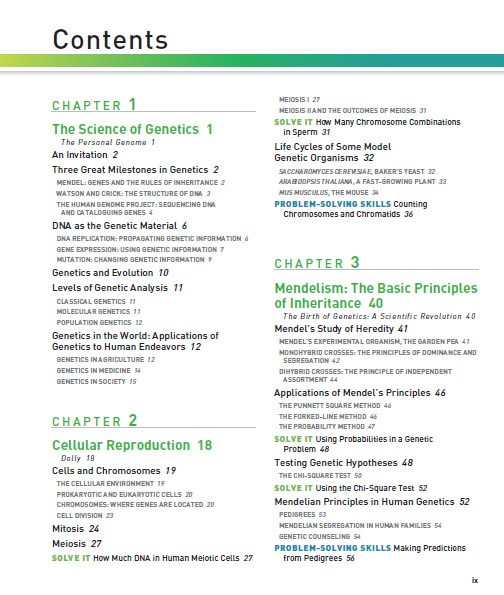
\includegraphics[width=0.5\textwidth]{contents01.png}}
\caption{Complex table of contents layout.}
\label{fig:toc}
\end{figure}


\begin{lstlisting}
\renewcommand\l@chapter[3]{%
  %#1 number and title  #2 page number
  \ifnum \c@tocdepth >\m@ne
    \addpenalty{-\@highpenalty}%
    \vskip 1.0em \@plus\p@
    \setlength\@tempdima{1.5em}%
    \begingroup
      \parindent \z@ \rightskip \@pnumwidth
      \parfillskip -\@pnumwidth
      \leavevmode
      \advance\leftskip\@tempdima
      \hskip -\leftskip
      \vbox{\raggedright#1\vskip1pt%
      \hrule width3cm height0.4pt}\par
      #2
      \penalty\@highpenalty
    \endgroup
  \fi}
\end{lstlisting}

\begin{lstlisting}
% define three parameters the chapter number, title separate
\renewcommand\l@chapter[3]{%
  %#1 number and title  #2 page number
  \ifnum \c@tocdepth >\m@ne
    \addpenalty{-\@highpenalty}%
    \vskip 1.0em \@plus\p@
    \setlength\@tempdima{1.5em}%
    \begingroup
      \parindent \z@ \rightskip \@pnumwidth
      \parfillskip -\@pnumwidth
      \leavevmode
      \advance\leftskip\@tempdima
      \hskip -\leftskip
      \vbox{\raggedright#1\vskip1pt%
      \hrule width3cm height0.4pt}\par
      #2
      \penalty\@highpenalty
    \endgroup
  \fi}
\cxset{chapter color=thegreen}
\l@chapter{\color{\chaptercolor@cx}\bfseries\chaptername\hskip1em\thechapter}{A Chapter Title}{12}
\end{lstlisting}


\subsection{Images in the TOC}
Figure \ref{fig:tocsteward} shows another |TOC| this time from a mathematics textbook. This is a much more complicated layout and includes images.

If we take a similarly flexible approach of redefining l@chapter we can try and format the toc shown in Figure \ref{fig:tocsteward}.

\begin{figure}[tp]
\centering

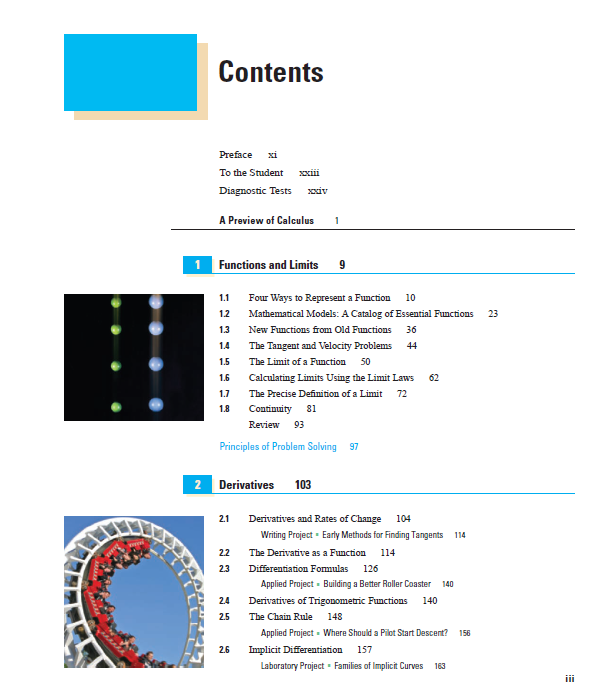
\includegraphics[width=0.8\textwidth]{contents02.png}
\caption{Complex table of contents layout.}
\label{fig:tocsteward}
\end{figure}



\begin{lstlisting}
\renewcommand\l@chapter[3]{%
  %#1 number and title  #2 page number
  \ifnum \c@tocdepth >\m@ne
    \addpenalty{-\@highpenalty}%
    \vskip 1.0em \@plus\p@
    \begingroup
      \parindent \z@
      \leavevmode
      \vbox{\raggedright\colorbox{blue}{\color{white}\bfseries\sffamily#1} #2\qquad  #3\vskip0pt%
      \color{blue}\hrule width0.7\textwidth height0.4pt}\par
      \penalty\@highpenalty
    \endgroup
  \fi}
\end{lstlisting}

\begin{lstlisting}
% define three parameters the chapter number, title separate
\cxset{
  toc chapter name/.store in=\chaptername,
  toc chapter name color/.code=\gdef\tocchapternamecolor@cx{#1},
  toc title color/.store in=\toctitlecolor@cx,
  toc title font-weight/.store in=\toctitlefontweight@cx,
  toc title before/.store in=\toctitlebefore@cx,
  toc title after/.store in=\toctitleafter@cx,
  toc after pagenumber/.store in=\tocafterpagenumber@cx,
}
\cxset{toc title color=theblue,  %interfers with links
       toc title font-weight=\fontfamily{ptm}\selectfont\bfseries ,
       toc title before=\hspace*{0.5em},
       toc title after=\hspace*{1.5em},
       toc after pagenumber=,
}

\renewcommand\l@chapter[3]{%
% #1 number #2
%  title  #2 page number
  \ifnum \c@tocdepth >\m@ne
    \addpenalty{-\@highpenalty}%
    \vskip 1.0em \@plus\p@
    \begingroup
      \parindent \z@
      \leavevmode
      \vbox{\raggedright\colorbox{blue}{\color{white}%
             \sffamily#1 }%
%% title formatting
        {\toctitlebefore@cx\color\toctitlecolor@cx\toctitlefontweight@cx%
          #2%
          \toctitleafter@cx}% font info
          #3\tocafterpagenumber@cx\vskip0pt%
              \color{blue}
              \hrule width0.7\textwidth height0.4pt}\par
      \penalty\@highpenalty
    \endgroup
  \fi}

\cxset{chapter color=thegreen}
\l@chapter{12}{A Chapter Title}{\thepage}%where is page number coming?numberline

\l@chapter{12}{A Chapter Title}{\thepage}
\end{lstlisting}


The above method of redefinition is a bit more flexible and can be extended to cover all cases that do not fall broadly with the standard class provisions. Any layout is possible.


\section{Writing the Table of Contents Entries}

So far we have examined the reading of the ToC file and next we need to understand the writing operation
to the ToC. If we have to ensure that information survives we need to write it to the file. This is done via two macros.




\begin{macro}{\addcontentsline}
The \cs{addcontentsline}\marg{table}\marg{type}\marg{entry} command allows the user to add an entry to a table of contents. The command adds the entry
\cs{contentsline}\marg{type}\marg{entry}\marg{page} to the \marg{.lot} file.
\end{macro}

\begin{teX}
 \addcontentsline{toc}{chapter}%
       {\protect\numberline{\thechapter}#1}
\end{teX}

\startlineat{144}
\begin{teX}       
 \long\def\addtocontents#1#2{%
 \protected@write\@auxout
 {\let\label\@gobble \let\index\@gobble \let\glossary\@gobble}%
 {\string\@writefile{#1}{#2}}}
\end{teX}

\begin{teX}
\def\addcontentsline#1#2#3{%
  \addtocontents{#1}{\protect\contentsline{#2}{#3}{\thepage}}}

\def\contentsline#1{\csname l@#1\endcsname}
\end{teX}

Of course the above are widely modified by the hyperref package and we should not touch them!

